\documentclass[a4paper,10pt]{article}
\usepackage[utf8]{inputenc}
\usepackage{datetime}
\usepackage{listings}
\usepackage{graphicx}
\newdate{date}{21}{04}{2017}
\date{\displaydate{date}}

\title{Homework 4\\Marlen Akimaliev\\BIL622-Numerical Analysis II}
%\author{Share\LaTeX}

\begin{document}

\maketitle

\section{Problem}
Solve the following Boundary Value Problem:\\
$x^2 \times y''-x \times y = 3 \times x^3$\\
$y(1) = 2$\\
$y(2) = 9$\\
Use shooting method for solution.
\section{Solution}
In order to solve second order BVP problem it has to be converted into a first order system of two equations:\\
Higher order differential equations can be written as a system with a very simple change of variable.  We’ll start by defining the following two new functions.\\
$x_1(t) = y(t)$\\
$x_2(t) = y'(t)$\\
If we differentiate both sides of these we get;\\
$x_1'=y'=x_2$\\
$x_2'=y''=(3\times x^3 + x \times y')/x^2=(3\times x^3 + x \times x_1)/x^2$\\
Putting all of this together gives the following system of differential equations.\\
$x_1' = x_2$, $x_1(1)=2$\\
$x_2'=(3\times x^3 + x \times x_1)/x^2$, $x_1(2)=9$\\
Following is the table after getting results at the range[2,9].
\begin{center}
\begin{tabular}{ |c|c| } 
 \hline
 $t$ & $x$\\
\hline
 $2.0$ & $2.0000000000000000$\\
 $2.8$ & $-13.4076702532885363$\\
 $3.6$ & $-26.5513372930734732$\\
 $4.3$ & $-37.6932727986715363$\\
 $5.1$ & $-46.1898472357814711$\\
 $5.9$ & $-50.8412316172525038$\\
 $6.7$ & $-49.9920471001467845$\\
 $7.4$ & $-41.5416864109323285$\\
 $8.2$ & $-22.9134425699207362$\\
 $9.0$ & $9.0000000000004121$\\
 \hline
\end{tabular}
\end{center}
Following Python code \cite{gordon} is used to evaluate values and plot the graph.
\begin{lstlisting}[language=Python]
import numpy
def shoot( f, a, b, z1, z2, t, tol ):
    from diffeq import rk4
    max_iter = 25   # Maximum number of shooting iterations
    n = len( t )    # Determine the size of the arrays we will generate
    y = rk4( f, [a,z1], t )
    w1 = y[n-1,0]
    for i in xrange( max_iter ):
        y = rk4( f, [a,z2], t )
        w2 = y[n-1,0]
        if abs( b - w2 ) < tol:
            break
        z1, z2 = ( z2, z2 + ( z2 - z1 ) / ( w2 - w1 ) * ( b - w2 ) )
        w1 = w2
    if abs( b - w2 ) >= tol:
        print "\a**** ERROR ****"
        print "Maximum number of iterations (%d) exceeded" % max_iter
        print "Returned values may not have desired accuracy"
        print "Error estimate of returned solution is %e" % ( b - w2 )
    return y[:,0]

if __name__ == "__main__":

    import math
    from pylab import *
    a = 2
    b = 9
    n1 = 10
    t1 = linspace( a, b, n1 )
    # Compute shooting method solutions
    def f(x,t):
        return array( [x[1], (3*t**3+t*x[0])/t**2] )
    xs1 = shoot( f, 2, 9, 1.0, 10.0, t1, 1e-5 )
    # Prepare for display; set interactive mode to true so each plot
    # is shown as it is generated
    interactive( True )
    for p1, p2 in list(zip(t1, xs1))[::1]:
    	print("%4.1f %10.16f" % (p1, p2))
    # Plot solutions
    plot( t1, xs1, 'ro')
    title( 'Shooting Method' )
    xlabel( "t" )
    ylabel( "x" )
    #legend( ( '%3d points' % n1, '%3d points' % n2 ), loc='lower right' )
    savefig( '1_2.eps', fmt='EPS', dpi=100 )
    draw()
    z = raw_input( "Press ENTER to quit..." )
\end{lstlisting}
If we try to plot these values as a graph result is as follows:
\begin{figure}[ht]
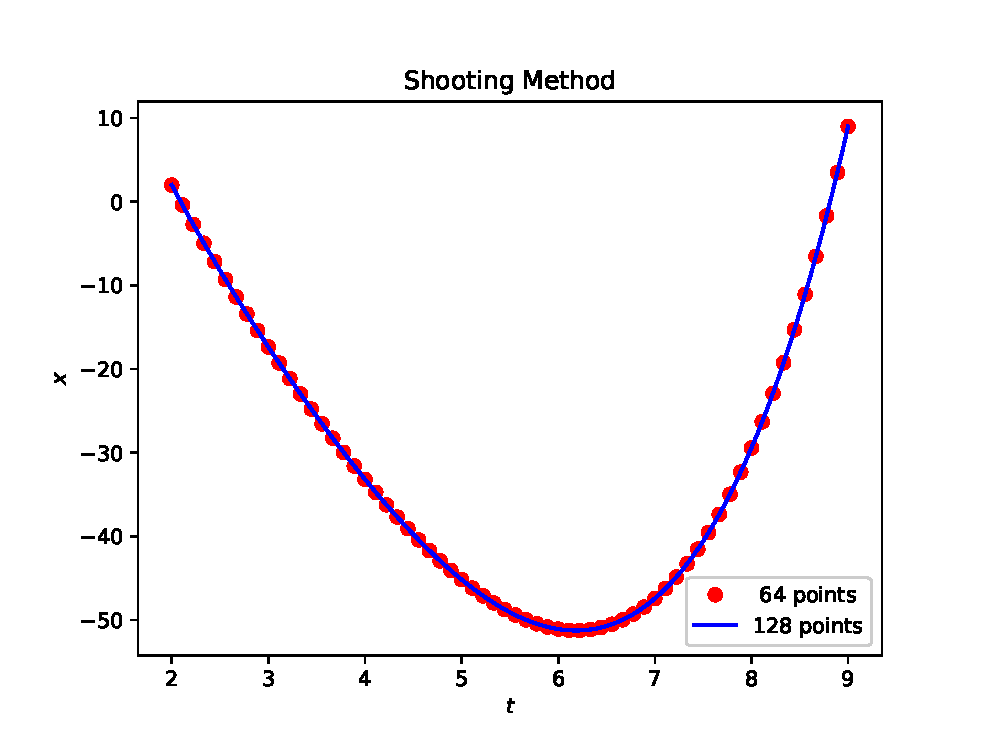
\includegraphics[width=8cm]{1_2.eps}
\end{figure}

\medskip

\begin{thebibliography}{9}
\bibitem{gordon} MAT342/CPS342 Python Demos, gordon.edu, \\\texttt{http://www.math-cs.gordon.edu/courses/ma342/python/bvp.py}
\end{thebibliography}

\end{document}
